\begin{figure}[t]
    \centering
    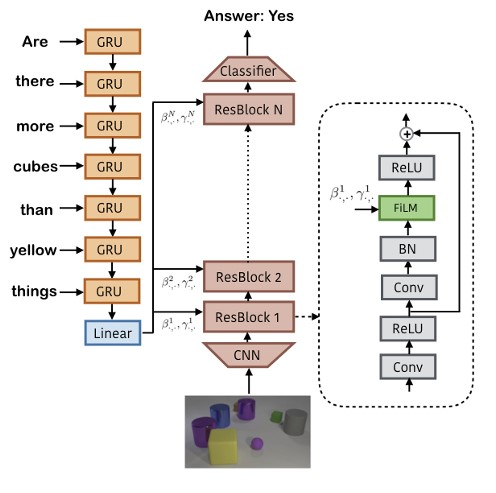
\includegraphics[width=0.6\textwidth]{figures/images/ch2/film_architecture.jpg}
    \caption{Proposed integration of the FiLM conditioning layer. Here, the Linear Modulation is applied to modify the activation maps of the ResNet blocks, while a linear layer generates the modulation coefficients $\beta$ and $\gamma$ based on the embedding derived from the textual prompt. This enables the model to conditionally adjust the activation maps according to the context provided by the input query}
    \label{fig:film_architecture}
\end{figure}
